% !TeX program = pdflatex
\documentclass[tikz,border=8pt]{standalone}
\usepackage{tikz}
\usetikzlibrary{calc,positioning}
\definecolor{FigureBlue}{HTML}{2563EB}
\definecolor{FigureOrange}{HTML}{EA580C}
\begin{document}
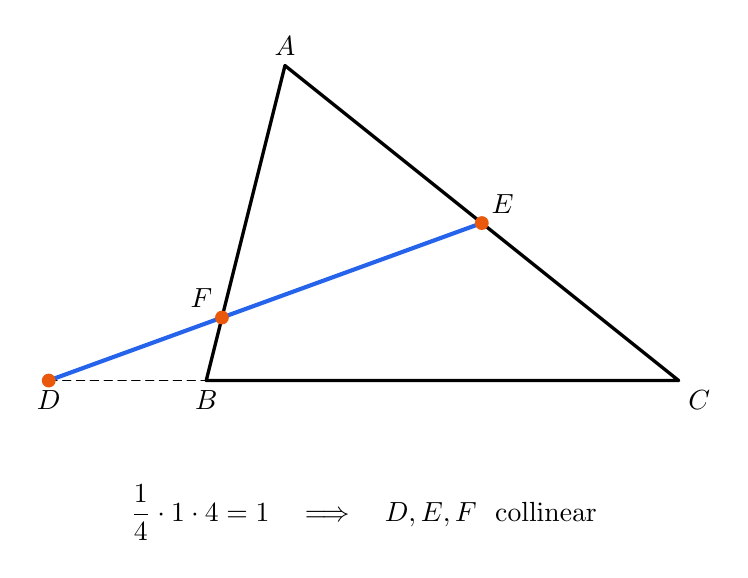
\begin{tikzpicture}[line cap=round,line join=round]
  \coordinate (A) at (1,4);\coordinate (B) at (0,0);\coordinate (C) at (6,0);
  \coordinate (D) at (-2,0);\coordinate (E) at ($(C)!.5!(A)$);\coordinate (F) at ($(A)!.8!(B)$);
  \draw[line width=1.2pt] (A)--(B)--(C)--cycle;
  \draw[densely dashed] (D)--(B);
  \draw[FigureBlue,line width=1.5pt] (D)--(E);
  \foreach \P in {D,E,F}{\fill[FigureOrange] (\P) circle (2.5pt);}
  \node[above] at (A) {$A$};\node[below] at (B) {$B$};\node[below right] at (C) {$C$};
  \node[below] at (D) {$D$};\node[above right] at (E) {$E$};\node[above left] at (F) {$F$};
  \node[below=12mm] at (2,0) {$\displaystyle\frac14\cdot1\cdot4=1\quad\Longrightarrow\quad D,E,F\ \hbox{ collinear}$};
\end{tikzpicture}
\end{document}
